\documentclass[border=1pt]{standalone}
\usepackage{tikz}
\usepackage{tikz-3dplot}

\begin{document}
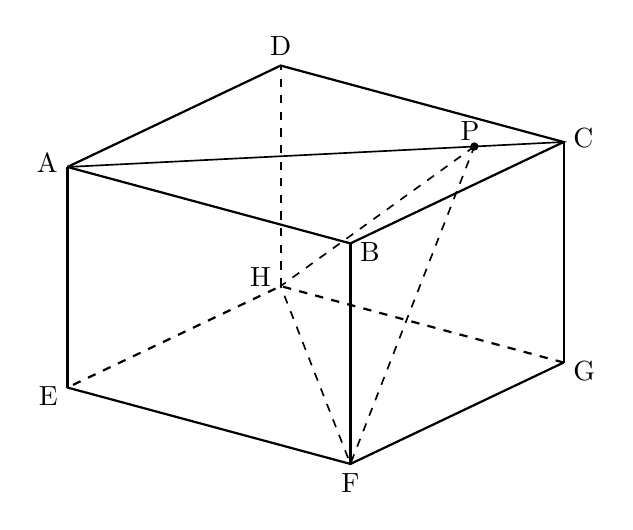
\begin{tikzpicture}
    \tdplotsetmaincoords{69}{127}
    \begin{scope}[tdplot_main_coords]
        
        % パラメータの定義
        \pgfmathsetmacro{\X}{4.5}
        \pgfmathsetmacro{\Y}{\X}
        \pgfmathsetmacro{\Z}{2*\X/3}
        \pgfmathsetmacro{\da}{0.12*\X}
        \pgfmathsetmacro{\db}{0.25*\X}
        \pgfmathsetmacro{\dc}{0.05*\X}

        % 頂点の座標の定義
        \coordinate (H) at (0,0,0); 
        \coordinate (E) at (\X,0,0); 
        \coordinate (F) at (\X,\Y,0);
        \coordinate (G) at (0,\Y,0);
        \coordinate (D) at (0,0,\Z);
        \coordinate (A) at (\X,0,\Z);
        \coordinate (B) at (\X,\Y,\Z);
        \coordinate (C) at (0,\Y,\Z);
        \coordinate (P) at ($(A)!0.82!(C)$);

        % 頂点のラベル
        \node[left, yshift=\db mm] at (H) {H};
        \node[left, yshift=-\db mm] at (E) {E};
        \node[below] at (F) {F};
        \node[right, yshift=-\db mm] at (G) {G};
        \node[above] at (D) {D};
        \node[left, yshift=\da mm] at (A) {A};
        \node[right, yshift=-\db mm] at (B) {B};
        \node[right, yshift=\da mm] at (C) {C};
        \node[above, xshift=-\da mm, yshift=-\da mm] at (P) {P};

        % 線・点の描画
        \draw [thick] (E) -- (F) -- (G);
        \draw [thick] (A) -- (B) -- (C) -- (D) -- (A);
        \draw [thick] (E) -- (A);
        \draw [thick] (F) -- (B);
        \draw [thick] (G) -- (C);
        \draw [thick,dashed] (H) -- (D);
        \draw [thick,dashed] (G) -- (H) -- (E);
        \draw [semithick] (A) -- (C);
        \draw [semithick,dashed] (P) -- (H) -- (F) -- (P);
        \fill (P) circle (1.5pt);
    
    \end{scope}
 
\end{tikzpicture}
\end{document}
